%!TEX root = these.tex

%\chapterstar{INTRODUCTION}
% Pour des renseignements sur \chapterstar : voir le fichier macros.tex

\chapterstar{Introduction} % "*" pour que l'introduction ne s'affiche pas dans la table des matières, sinon elle s'y affichera comme un chapitre d
% \mtcaddchapter
% \addstarredpart{Introduction} % Pour ajouter une partie ("part") fictive dans la table des matières
% \mtcaddpart
% \markboth{Introduction}{Introduction}  %% header manuel car sinon, ils me marquent le header du dernier \chapter{?} (on est dans un \chapter*{?} )
\selectlanguage{francais}


\section*{Contexte et problématique}

Il est possible de diviser la biologie structurale et donc l'étude théorique de structures moléculaires en trois activités principales organisées selon le processus séquentiel suivant : (1) l'\textbf{expérimentations}, (2) la \textbf{modélisation moléculaire} et (3) la \textbf{simulation moléculaire} des structures 3d. Chacune de ces étapes met en jeu des outils de visualisation et d'analyse permettant d'étudier les données générées, de les interpréter pour les étapes suivantes et enfin de produire de nouvelles connaissances et d'établir de nouvelles hypothèses scientifiques. Plusieurs itérations de ce processus sont nécessaires pour caractériser les mécanismes en jeu dans un complexe moléculaire dans son environnement, chaque nouveau processus prenant comme données d'entrée une partie des résultats générés par l'analyse des données du processus précédent.

\begin{figure}[h]
  \centering
  {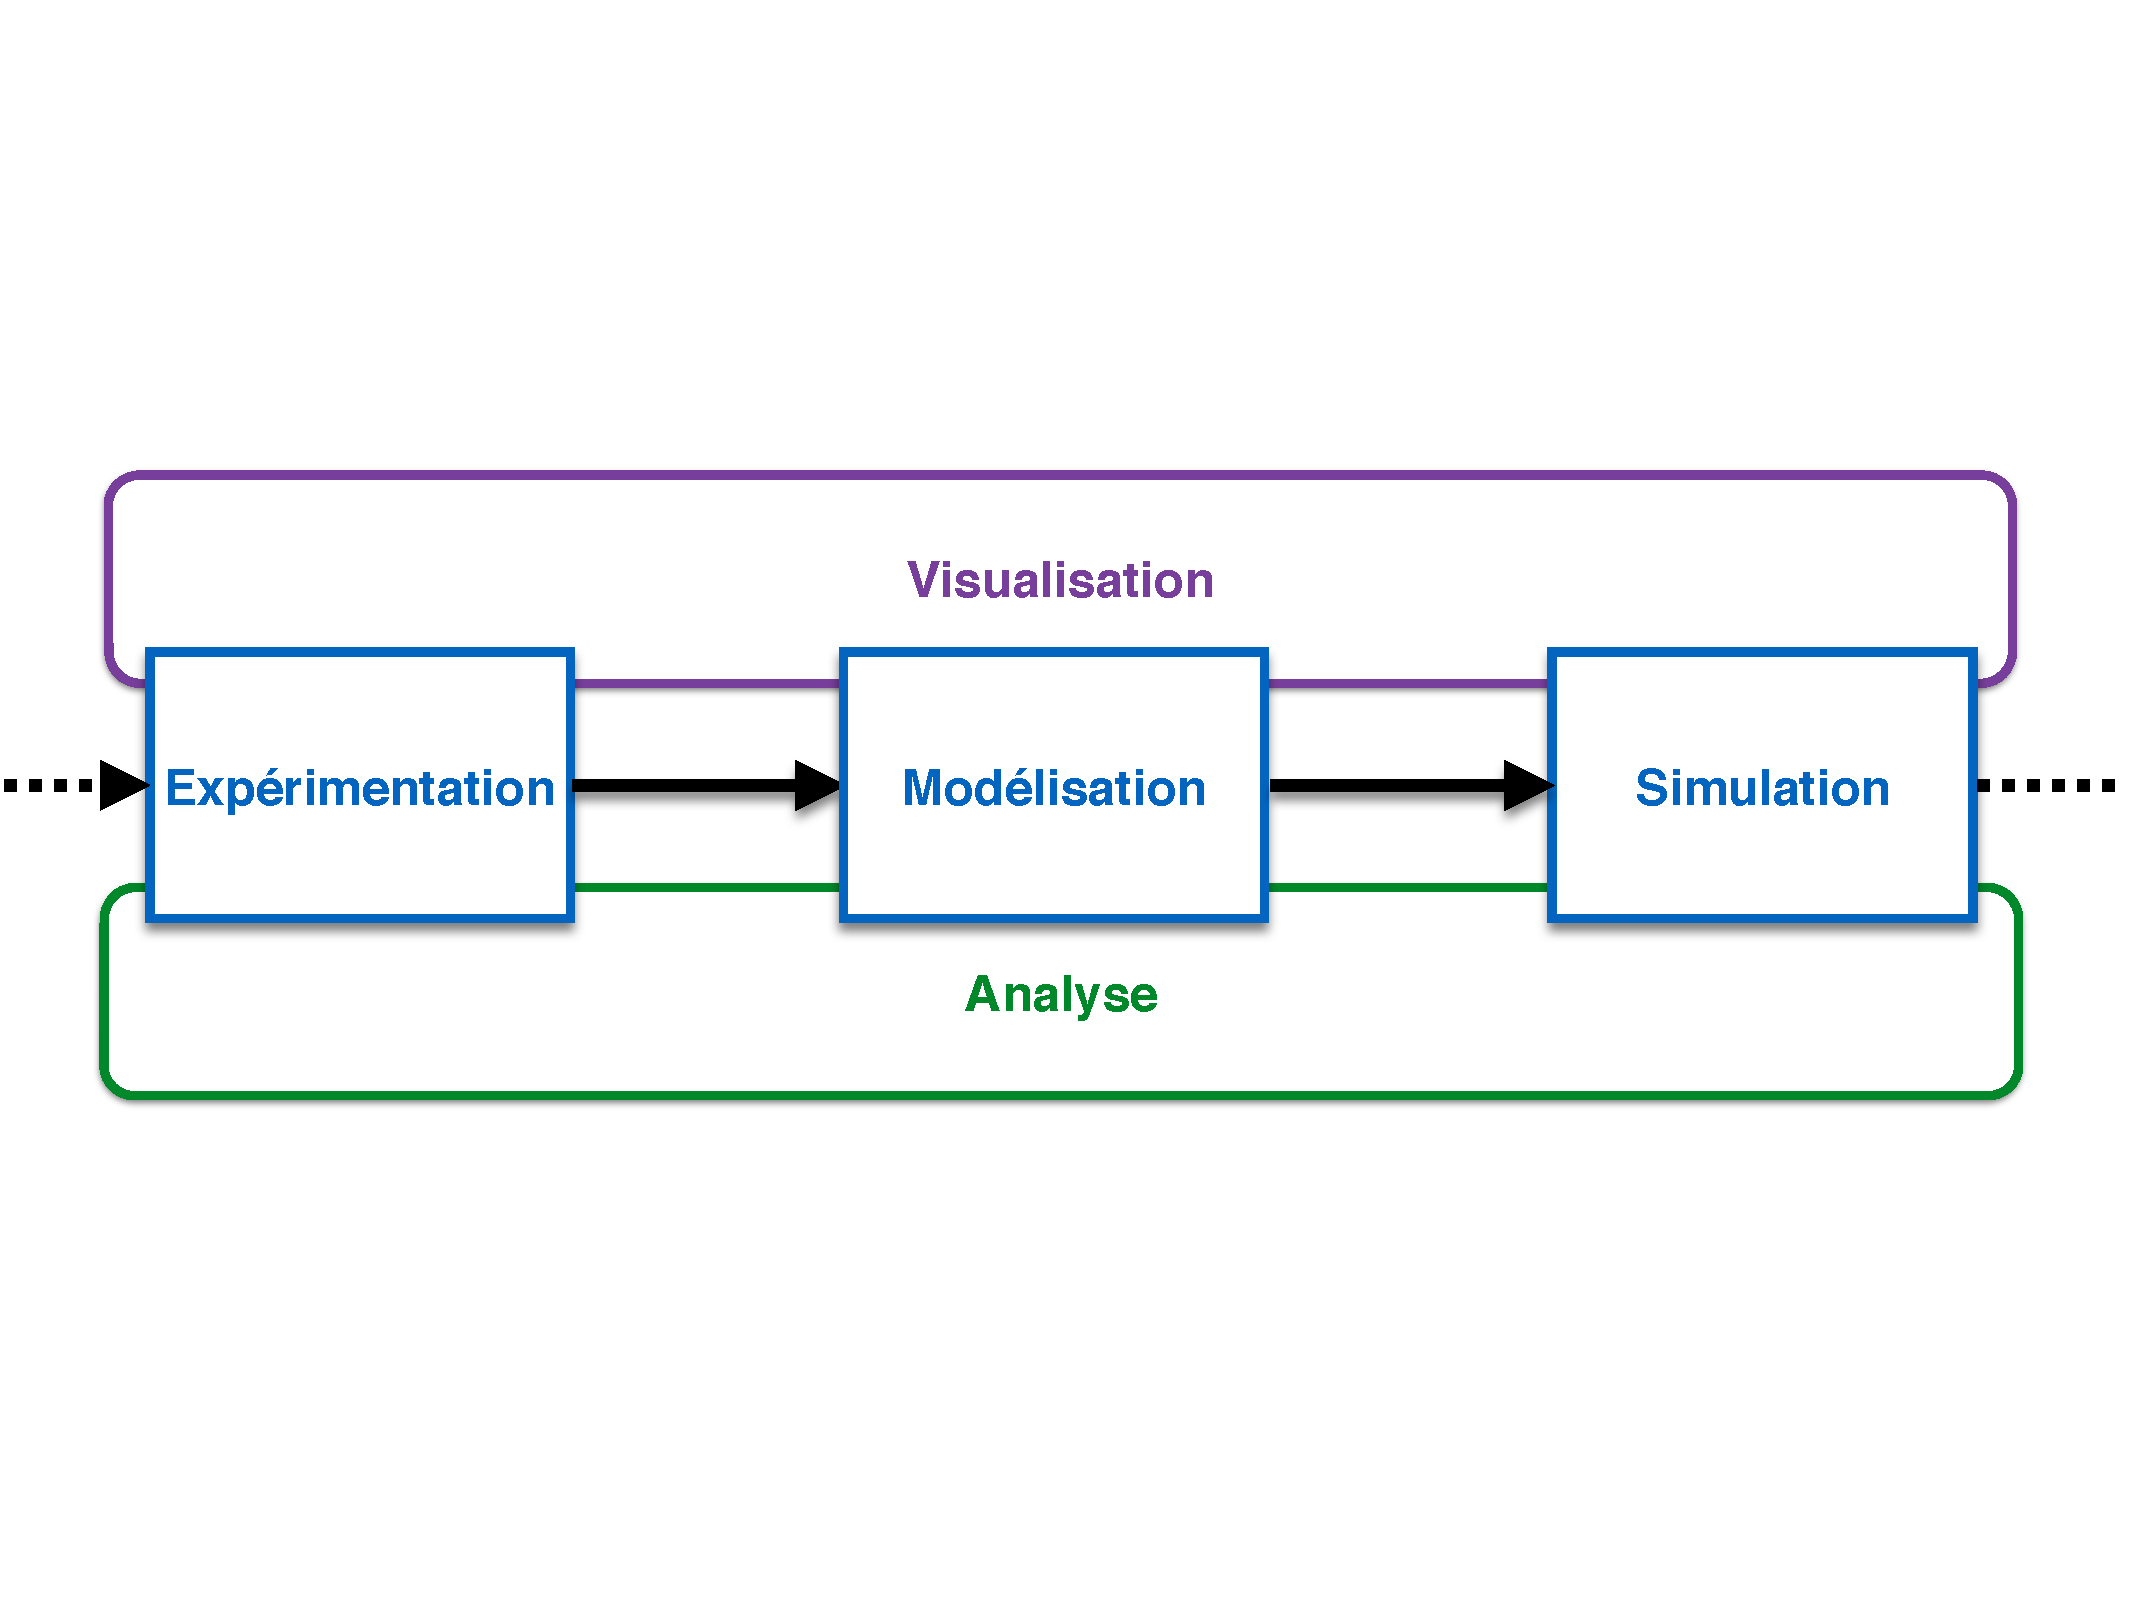
\includegraphics[width=.75\linewidth]{./figures/ch1/process_bio_struct}}
    \caption[Schéma du processus itératif d'étude d'une structure moléculaire en biologie structurale.]{\it Schéma du processus itératif d'étude d'une structure moléculaire en biologie structurale. Les trois grandes étapes sont représentées en bleu, les outils de visualisation et d'analyses présents tout au long du processus sont représentés respectivement en violet et vert.}
  \label{Fig:process_bio_struct}
  \hspace{0.2cm}
\end{figure}

Au sein de ce processus, la performance croissante des outils de calcul informatique entraîne aujourd'hui la génération de volumes de données considérables, en particulier dans la phase de simulation. De ce fait, les modèles de complexes moléculaires étudiés sont beaucoup plus gros et sont caractérisés par des résultats de plus en plus précis et détaillés. Aujourd'hui, l'efficacité croissante des programmes de simulation numérique moléculaire conduit à la production des données de trajectoires moléculaires, suite de modèles 3d décrivant l'évolution temporelle de structures moléculaires, pouvant atteindre plusieurs millions de particules à une précision atomique \cite{sanbonmatsu2013molecular}. En parallèle, la performance des outils de manipulation et de visualisation moléculaire n'a pas progresser de manière suffisamment significative pour absorber l'évolution des ressources de calcul et de stockage dédiées à la simulation moléculaire. L'étape de visualisation n'est pas la seule victime de l'amélioration des moyens de calcul. En effet, cette efficacité croissante des outils de simulation n'a pas été compensée par une augmentation suffisante des moyens d'analyse et la quantité générée de données est bien souvent très supérieure à la quantité de données pouvant être traitée par les experts scientifiques. De même, les capacités de calcul ont depuis longtemps dépassé les capacités de stockage, pourtant elles-mêmes en croissance forte  \cite{zimmerman2014data}. \textbf{Visualiser, modéliser, et analyser des complexes moléculaires de très grande taille est donc devenu un enjeu crucial en biologie moléculaire}. Enfin, la taille des données impacte directement l'efficacité et la rapidité des échanges de données entre les centres de calcul et les laboratoires de biologie. La minimisation de la quantité de données à échanger, à stocker et à analyser constitue une problématique importante pour les laboratoires.

L'approche dite \textit{In Situ} répond à cette dernière problématique, en déportant les étapes de rendu graphique et d'analyse dans les centres de calcul \cite{kuhlen2011parallel,ma2009situ}. Cette approche suppose cependant de prévoir les analyses et les représentations visuelles qui seront nécessaires à la compréhension du phénomène. Les résultats de simulation, les représentations visuelles et les résultats d'analyse de la trajectoire sont ensuite analysés par l'expert en restant sur les centres de calcul. Cette méthodologie est cependant très difficile à mettre en pratique, car le choix des analyses requises dépend du résultat de la simulation que l'expert visualise en choisissant des modalités de visualisation, par ailleurs spécifique à chaque phénomène étudié. Planifier les analyses et les rendus graphiques pourrait donc techniquement résoudre cette problématique de stockage et de transferts des données massives, mais ne correspond pas aux usages et aux contraintes dans un domaine dans lequel l'expert intervient nécessairement à chaque étape du processus. Pour minimiser les données échangées, \textbf{il s'agit donc de rapprocher les étapes de simulation, de visualisation, d'analyse tout en permettant à l'expert de pouvoir effectuer des visualisations et des analyses à la demande sur le lieu de simulation.}

%L'approche de simulation moléculaire tente de recentrer l'expert au centre de son objet d'intérêt par des solutions technologiques de haute performance permettant le suivi et le contrôle en temps interactif d'un phénomène étudié pendant une une simulation en cours \cite{dreher_interactive_2013}. Cette approche souffre cependant d'une limitation importante en terme de  performance lorsque elle est utilisée en dehors d'infrastructures lourdes dédiées aux communications entre les centres de calcul et les laboratoires, la quantité de données échangée étant souvent supérieure aux capacités d'échange des réseaux standards. Si elle permet de recentrer l'expert dans la boucle de simulation et de visualisation, elle n'a pas pour objectif de fournir des solutions pour analyser de grosse quantité de données.

%Le positionnement de l'expert scientifique au centre de la boucle de décision passe donc par la mise en place d'éléments d'analyse et de visualisation liés de façon à ce que l'utilisateur puisse appréhender le phénomène observé dans son ensemble pour intervenir à tout instant du processus de simulation. 

%L'articulation entre visualisation et analyse est donc primordiale et doit passer par un espace de travail commun et mixte qui rassemblera ces deux étapes du processus de biologie structurale. \textbf{Il s’agit concrètement de présenter de manière conjointe, simultanée et interactive les structures moléculaires et leurs résultats d'analyses}


La biologie structurale a toujours su intégrer au sein de chacune de ses étapes les résultats du domaine des sciences et technologie de l'information. Du traitement des signaux des méthodes expérimentales jusqu'à la visualisation de structures 3d, les avancées technologiques ont toujours été rapidement intégrées au coeur de ses outils. Des concepts issus de la réalité virtuelle, comme la stéréoscopie ont rapidement été utilisés pour mieux appréhender des contenus moléculaires intrinsèquement tridimensionnels \cite{van2000immersive,stone_immersive_2010,odonoghue_visualization_2010}. La réalité virtuelle est aussi associée à un espace de travail très important avec un point de vue adaptatif facilitant l'exploration de complexes moléculaires de grande taille. Enfin, des dispositifs d'interaction 3d permettant d'interagir et de ressentir les forces en jeux dans un système moléculaire, hier confidentiel, sont désormais utilisés et intégré dans les usages et les outils de la biologie moléculaire. On peut donc s'attendre à ce que le domaine de la biologie moléculaire continue d'intégrer dans ses usages les nouvelles technologies et dispositifs de réalité virtuelle, en particulier les dispositifs financièrement très abordable donnant accès à une immersion de grande qualité sur le lieu de travail des experts.

%Elle est associée à des espaces d'affichage où l'utilisateur dispose d'un point de vue dynamique autour de  l'objet observé (systèmes CAVE, murs d'écrans, etc...), ou par des dispositifs de taille plus réduite et portable mais à travers lesquels l'utilisateur peut également percevoir un monde virtuel à 360 degrés grâce à un suivi de l'orientation de sa tête (casques stéréoscopiques, etc...). Les canaux auditifs et tactiles sont également au centre des considérations de la RV. L'audio 3d permettant de simuler des sources audio dans un environnement 3d autour de l'utilisateur et les retours haptiques associés à certains dispositifs d'interaction permettent de simuler une dimension tangible lors de l'interaction de l'utilisateur avec l'environnement virtuel. Ces canaux constituent tout deux des approches supplémentaires pour immerger davantage l'utilisateur au sein de données virtuelles qu'il étudie.

%La RV offre en effet une perception stéréoscopique, atout pour une meilleure compréhension des données moléculaires intrinsèquement tridimensionnelles . Elle est également le support de contextes interactifs favorisant la manipulation directes de données virtuelles. Elle se caractérise par des interactions directes avec les objets virtuels présentés via des gestes et/ou par des commandes vocales .

Cependant, l'immersion comporte des limites qu'il convient d'adresser avant de pouvoir constituer un outil récurrent en la biologie structurale. La navigation au sein de dispositifs immersifs dans des données abstraites est un premier obstacle. Le mal du simulateur, souvent provoqué par l'activité de navigation dans les scènes virtuelles immersives réalistes et amplifié lors de l'exploration de données abstraites comme les données scientifiques, dégrade l'expérience de l'utilisateur, en particulier dans les dispositif immersif récent et grand public comme les HMD. \textbf{Des paradigmes de navigation adaptés aux contenus moléculaires abstraits et à la tâche de l'expert sont un pré-requis à l'intégration de l'immersion en biologie moléculaire}.

%Plusieurs études ont montré que ce mal du simulateur possède plusieurs points communs avec le mal des transports \cite{laviola_jr_discussion_2000}. De la même façon que pour le mal des transports, dans un environnement immersif, le cerveau dissocie difficilement les retours visuels de la scène virtuelle aux sollicitation physiques incohérentes ou inexistantes prenant place au même instant. Cette dissociation de la sollicitation du système vestibulaire par rapport au système perceptif \cite{reason1975motion} entraîne chez certaines personnes l'apparition de symptômes qui peuvent aller de légères sensations d'inconfort à de plus importants troubles de l'équilibre ou de nausées. Les paradigmes de navigation en condition immersive sont multiples mais ont souvent été développé pour répondre à des contraintes de navigation dans des scènes réalistes et ne parviennent donc pas à répondre aux attentes d'efficacité requises au sein de scènes virtuelles dont les informations proposées sont de nature différente \cite{trellet_content-guided_2014}. La différence de l'approche de navigation entre les scènes réalistes et abstraites peut s'expliquer par: 1) une absence de repères spatiaux dans les scènes abstraites où les données scientifiques ne sont généralement pas exposées au sein d'un environnement mais dans un espace vide monochromatique, 2) une absence de notion d'orientation, sans haut ni bas, 3) une exploration centrée sur un objet unique au centre de l'attention. 


%L'intégration des analyses à la visualisation, dans l'optique de permettre une compréhension globale de l'ensemble des paramètres et données de sa simulation à l'utilisateur constitue un \textit{deuxième obstacle} à franchir pour l'implémentation de la biologie structurale au sein d'environnements immersifs.
%Les dispositifs adaptés aux espaces immersifs existent mais ils ne peuvent répondre à l'intégralité du large spectre de tâches propres à la biologie structurale. Parmi ces tâches, la sélection, le changement de rendu graphique, le mouvement et l'accès aux informations sont plusieurs actions indispensables en visualisation moléculaire. A ces tâches s'ajoutent toutes les tâches propres aux espaces d'analyse et permettant d'interagir avec des représentations analytiques de propriétés ou calculs statistiques accompagnant une simulation. 
%\textbf{Afin d'optimiser la couche d'interaction entre l'utilisateur et les espaces de travail, il est donc nécessaire de mettre en place une méthode robuste permettant à la fois d'anticiper et de simplifier les étapes d'interaction pour l'exécution de chaque tâche.}


Par ailleurs, les interactions dans un environnement immersif ne peuvent être être médiatisées par les dispositifs classiques comme la souris et le clavier. Elles sont mis de côté au profit d'interactions directes avec les objets virtuels présentés \textit{via} des gestes et/ou par des commandes vocales. Par ailleurs, les environnements immersifs imposent un contexte d'interaction unique et homogène, avec un espace de travail non fenêtré. Pour répondre à ces contraintes propres aux environnement immersifs et les rendre opérationnels pour le domaine de la biologie moléculaire, \textbf{il s'agit de rapprocher les étapes de simulation, de visualisation, d'analyse dans un contexte interactif unique, en favorisant les interactions directes}.




%Plusieurs dispositifs adaptés aux espaces immersifs existent mais ils ne peuvent répondre efficacement au large spectre de tâches propres à la biologie structurale. Parmi ces tâches, la sélection, le changement de rendu graphique, le mouvement et l'accès aux informations sont plusieurs actions indispensables en visualisation moléculaire. A ces commandes s'ajoutent toutes les actions propres aux espaces d'analyse et permettant d'interagir avec des graphiques représentant les résultats d'analyse.  

% Afin de garantir une optimisation de la couche d'interaction entre l'utilisateur et les espaces de travail, il est donc nécessaire de mettre en place une méthode robuste permettant d'anticiper et de simplifier les étapes d'interaction permettant d'accomplir chaque tâche. 

% Afin de répondre aux différentes problématiques exposées précédemment, il fut nécessaire de prendre en compte deux contraintes supplémentaires. Ces contraintes, en filigrane tout au long de notre étude, ont motivé nos choix techniques pour assurer à l'utilisateur une expérience immersive de travail aussi efficace que dans des conditions standards de bureau.
% La première contrainte est la contrainte de temps réel que nous imposent la plupart des environnements immersifs lorsqu'il est question de rendu stéréoscopique s'adaptant au point de vue utilisateur. La réduction de la latence entre les mouvements de l'utilisateur et le rendu calculé pour la nouvelle position et orientation de l'utilisateur à chaque instant fut une  . Nous nous appuyons essentiellement sur des briques techniques et technologiques qui ont déjà prouvé leur efficacité pour le rendu 3d temps réel, il est donc nécessaire que nos apports, en particulier pour la navigation et l'exploration, ne soient pas un frein à l'immersion et au rendu temps réel qui lui est propre.
% La deuxième contrainte temporelle vient de la contrainte interactive inhérente à tout système où l'action de l'utilisateur induit un changement visuel ou structurel de la scène et des informations qu'il perçoit. Cette contrainte en temps interactif fut un point important du développement de notre liaison bi-latérale entre espace d'exploration et espace d'analyses. Ce temps interactif doit se rapprocher au maximum de ce que pourrait attendre l'utilisateur, en terme de retours sensoriels, lors du déclenchement d'une action. Il n'est souvent pas nécessaire que l'action voit sa réalisation s'effectuer en temps réel, c'est pourquoi nous parlerons de temps interactif.

 
\section*{Approche générale}

Motivés par le manque de paradigmes de navigation spécifiques pour domaine de la biologie structural, notre premier axe de travail s'est concentré sur le \textbf{développement de méthodes de navigation immersive basées sur le contenu et la tâche en biologie structurale}. Ces méthodes et paradigmes s'inspirent de  particularités géométriques souvent observés dans la plupart des complexes moléculaires : un agencement des sous-unités de façon symétrique \cite{goodsell_structural_2000}. Notre approche n'est néanmoins aucunement contrainte à des complexes moléculaires symétriques puisque toute structure particulière retrouvée au sein d'une molécule nous permet de mettre en place nos paradigmes de navigation. Grâce à ces paradigmes, tout au long de son exploration, l'utilisateur 1) garde un point de vue stable sur son complexe, 2) possède des repères spatiaux fixes afin de se situer dans la scène, 3) peut utiliser des chemins préférentiels qui respectent les deux conditions précédentes pour se déplacer pour atteindre des régions d’intérêt. Ces apports répondent respectivement aux problèmes de mal du simulateur pouvant être ressentis à cause: 1) d'une variation trop rapide de l'orientation de l'utilisateur par rapport à sa cible visuelle, 2) d'un dégradation de la conscience spatiale de l'utilisateur dans sa scène, 3) d'un trop grand nombre d'étapes ou de temps pour atteindre une région d'intérêt tout en gardant une conscience spatiale de la scène virtuelle. En contraignant la navigation autour de chemins répondant aux objectifs d'exploration, \textit{via} une restriction des directions du mouvement et des orientations de la caméra, nous fournissons des possibilités de navigation limitées mais adaptées aux interactions pouvant prendre place au sein des environnements immersifs. De la même manière, nous anticipons certaines tâches d'exploration en fournissant des paradigmes automatisant certains déplacements considérés comme habituels en exploration moléculaire. Comme l'immersion sera probablement intégrée de manière progressive dans les usages, nous avons souhaité parallèlement au développement de paradigmes de navigation immersive dédiés, profiter de la démocratisation des périphériques mobiles en une démarche parallèle afin de \textbf{concevoir des solutions de visualisation en immersion réduite et avec une perception de la profondeur des contenus moléculaires}. 

%%%%%%%%%%%%%%%%%%%%%%%%%%%%%%%%%%%%%%%%%%%%%%%%%%%%%%%%%%%%%%%%%%%%%%%%%%%%



%La première application de notre outil fut le contrôle de l'évolution d'une simulation moléculaire par un expert scientifique. Ce contrôle doit permettre d'appréhender la direction vers laquelle tend une simulation et mettre ainsi en évidence d'éventuelles évolutions ne respectant pas les contraintes imposées ou présentant des incohérences scientifiques notables. 

%Nous proposons un support mobile permettant de visualiser de façon simple et rapide l'état d'une simulation à travers une ou plusieurs photographies de la structure simulée. La légèreté des images utilisées pour ce rendu et le développement axé multi-plateforme de notre application, permet également son utilisation au sein de communications scientifiques diverses (journaux papier, journaux électroniques, actes de conférences, etc...) afin d’accroître la quantité d'information présentée. A la différence des images 2d habituelles, notre méthode permet un rendu pseudo-3d pour des illustrations complexes constituées de plusieurs couches et/ou affichant un objet désirant être affiché en profondeur. 
%L'importation d'objets 3d et leur exploration à la manière d'un visualiseur 3d sont également associées à l'application et permettent la manipulation de structures complètes de molécules. Deux méthodes permettent d'appréhender la structure du modèle 3d importé, le premier est basé sur une manipulation simple grâce à un ensemble de rotations et translations, le second propose lui d'utiliser le périphérique mobile à la manière d'une fenêtre sur un monde virtuel entourant l'utilisateur et qu'il peut regarder au travers de son périphérique.

%%%%%%%%%%%%%%%%%%%%%%%%%%%%%%%%%%%%%%%%%%%%%%%%%%%%%%%%%%%%%%%%%%%%%%%%%%%%%

Notre troisième sujet d'études donne les clés qui nous ont permises \textbf{de regrouper des espaces de visualisation et d'analyse dans un contexte interactif homogène grâce à une modélisation sémantique}, afin de raccourcir la boucle d'étude des données de simulation moléculaire et pour répondre à la fois aux nouveaux enjeux de la biologie moléculaire et aux contraintes des environnements immersifs. %Comme exposé précédemment, dans une situation en temps réel, un enjeu majeur est de réduire les données échangées entre les composants de simulation, de visualisation et d'analyse pour permettre à un utilisateur de contrôler ces trois composants au sein d'une même plateforme et en temps interactif. 
Nous avons été inspirés par les techniques de \textit{Visual analytics} visant à fournir de  l'interactivité entre plusieurs représentations d'un phénomène ou de ses analyses pour faciliter les corrélations\cite{kielman2009foundations}.
Pour ce faire, notre approche s'est basée sur la mise place d'une couche d'abstraction décrivant les données manipulées usuellement par les experts du domaine. Cette couche d'abstraction a pu être mise en place par la construction d'une description sémantique des concepts mis en jeu lors de la visualisation et l'analyse de structures moléculaires. Cette description fut l'objet de la définition d'une ontologie, afin de formaliser l'ensemble des concepts mis en jeu lors d'une session de travail en intégrant l'ensemble des connaissances que possèdent l'expert scientifique en biologie moléculaire \cite{berners2001semantic}. Cette représentation sémantique nous permet d'effectuer des liens interactifs entre les différentes représentations analytiques ou scientifiques d'objets d"intérêt présentés selon différentes modalités.

%Les utilisateurs possèdent, à travers l'ontologie mise en place, une suite de règles et de descriptions des concepts qu'ils vont manipuler, leur permettant à la fois de comprendre l'organisation de leurs informations scientifiques au sein de l'application mais également d'enrichir cette organisation via l'élargissement de l'ontologie. L'ontologie mise en place permet enfin de garder une homogénéité forte pour chaque nouvelle étude. En définissant les concepts pouvant être utilisés, elle impose en effet un formatage clair des données qui permet finalement un recoupage très aisé des données générées au sein de chaque base de données (dans le cas d'une base de données par cas d'étude) et assure ainsi leur inter-compatibilité.


\section*{Plan du manuscrit}

Notre travail étant à l'interaction entre la biologie moléculaire et l'informatique, nous avons porté une attention particulière pour présenter aux lecteurs des chapitres de présentation, nous l'espérons claire et concise, des différents domaines concernées, qui ne font pas nécessairement partie du domaine d'expertise du lecteur. Nous aborderons l'ensemble de nos contributions et les contextes dans lesquels ils s'inscrivent au travers de 5 chapitres distincts, le premier chapitre pouvant être lu rapidement par les lecteurs familiarisés à la biologie moléculaire, le second chapitre pouvant être lu rapidement par les lecteurs familiarisés à la réalité virtuelle.

Le \textbf{premier chapitre} fera un retour sur notre domaine d'application, la biologie structurale, à travers sa définition, ses usages et ses enjeux. Nous identifierons tout d'abord les acteurs et processus du domaine plus large que constitue la biologie moléculaire, nous concentrant principalement sur le coeur de la transformation de l'information génétique en acteurs du fonctionnement d'une cellule vivante. Cela nous amènera à cerner la place de la biologie structurale au sein de la biologie moléculaire. Les différentes méthodes et outils caractérisant la biologie structurale seront ensuite énumérées pour finalement énoncer ses limites et recenser ses nouveaux usages. 

Le \textbf{second chapitre} abordera le nouvel usage que constitue la notion d'immersion de l'utilisateur fournie par la Réalité Virtuelle. Nous définirons tout d'abord ce domaine à travers trois de ses principaux axes: l'immersion, l'interaction et la navigation. Ses apports à la biologie structurale sont ensuite discutés pour finalement identifier les limites actuelles de son application en biologie structurale.

Nous développerons dans le \textbf{troisième chapitre} nos contributions pour amener la dimension immersive au coeur de trois aspects importants de la biologie structurale : la diffusion au sein de la communauté de structures 3d, le contrôle rapide de l'état d'une simulation numérique moléculaire et l'exploration de complexes moléculaires.

Le \textbf{quatrième chapitre} sera consacré à la présentation de pistes scientifiques pouvant apporter des réponses concrètes aux limites actuelles de l'utilisation de la Réalité Virtuelle en biologie structurale. Parmi ces pistes, la visualisation analytique sera mise en avant à travers plusieurs de ses méthodes et techniques qui seront détaillées. Nous mettrons en avant l'apport de l'interactivité qu'elle introduit pour les tâches d'analyses et de visualisation moléculaire. Nous introduirons plus particulièrement comment l'interactivité entre ces deux tâches hétérogènes peut être offerte grâce à la création d'un cadre sémantique homogène. 

Finalement, le \textbf{cinquième chapitre} sera consacré à l'implémentation d'un prototype d'application rapprochant les espaces d'analyses et de visualisation au sein d'un même contexte interactif, adapté aux environnements immersifs en privilégiant les interactions directes. Nous montrerons comment les outils issus du web sémantique en modélisant conjointement les contenus moléculaires et les interactions possibles sur ces contenus, peuvent supporter le rapprochement des phases d'analyse et de visualisation. 